\section{Pentaho Data Integration}
Nas seções anteriores foi discutido um pouco das principais características de um Data Warehouse e do processo CRISP-DM. Nessa seção, será discutida a utilização do Pentaho Data Integration (PDI) no processo de ETL, como ela pode ser aplicada e suas principais características.
O PDI, também conhecido como Kettle, oferece diversas ferramentas para a extração de dados de fontes diversas, transformações, limpezas e de carregamento dos dados
\subsubsection{Arquitetura}
O \pdi é composto basicamente de quatro componentes:
\begin{itemize}
    \item Spoon: é uma aplicação desktop de interface gráfica para a criação de jobs e transformations. Permite a criação de processos de ETL sem a necessidade de programação;
    \item Pan: uma interface de linha de comando que pode ser usado para a execução de jobs;
    \item Kitchen: interface de linha de comando que pode ser usada para a execução de jobs;
    \item Carte: uma aplicação web que permite a utilização de um servidor de ETL remoto, fornecendo capacidades de execução remota similares ao servidor de Data Integration.
\end{itemize}
\subsubsection{Princípios de Design}
\citeauthor{kettle}(\citeyear{kettle}) diz que o Pentaho foi desenvolvido com alguns princípios de design fundamentais, eles são. Algumas experiências negativas levaram a essas decisões.

Ele é de fácil desenvolvimento, não é necessário se preocupar com instalação de software. Segundo \citeAuthorPageYear{kettle}, várias ferramentas baseadas em Java precisavam que o usuário especificasse explicitamente qual era o nome da Classe Java de Driver e a URL do JDBC, apenas para criar uma conexão com o banco de dados. O Kettle sempre tentou ficar longe desses problemas \citep{kettle}. Ele evita a necessidade de programar, toda linha de código adiciona complexidade e custo de manutenção ao projeto, então faz sentido não ter que lidar com isso \citep{kettle}.

Ele mantém as funcionalidades disponíveis na interface de usuário, \citeAuthorPageYear{kettle} diz que é possível realizar ETL por XML, repositório ou uma API. E todas essas opções também estão disponíveis em uma interface gráfica. Sem limitações de nomenclatura, as ferramentas de ETL precisam ser inteligentes para lidar com qualquer tipo de identificador, isso permite que a solução seja auto descritíva e reduzindo parcialmente a necessidade de documentação \citep{kettle}.

\citeAuthorPageYear{kettle} diz que permitir que qualquer pessoa veja o que está acontecendo nas várias partes de um processo de ETL é crucial, permite acelerar o desenvolvimento e reduzir o custo. Fluxo de dados flexível, o \pdi foi criado para ser o mais flexível possível, respeitando os fluxos que podem ser criados \citep{kettle}. Apenas mapear dados impactados, \citeAuthorPageYear{kettle} diz que um dos princípios fundamentais do Kettle é todos os campos que não são mapeados passam automaticamente para o próximo passo do processo, reduzindo assim o custo de manutenção.

\subsubsection{Processo}
Ao abrir o \pdi, ele apresenta a página inicial, como mostra na figura \ref{initialpdi}. Dessa tela é possível criar \textit{Jobs} e \textit{Transformations}, que serão explicados mais pra frente. 
\begin{figure}[H]
\centering
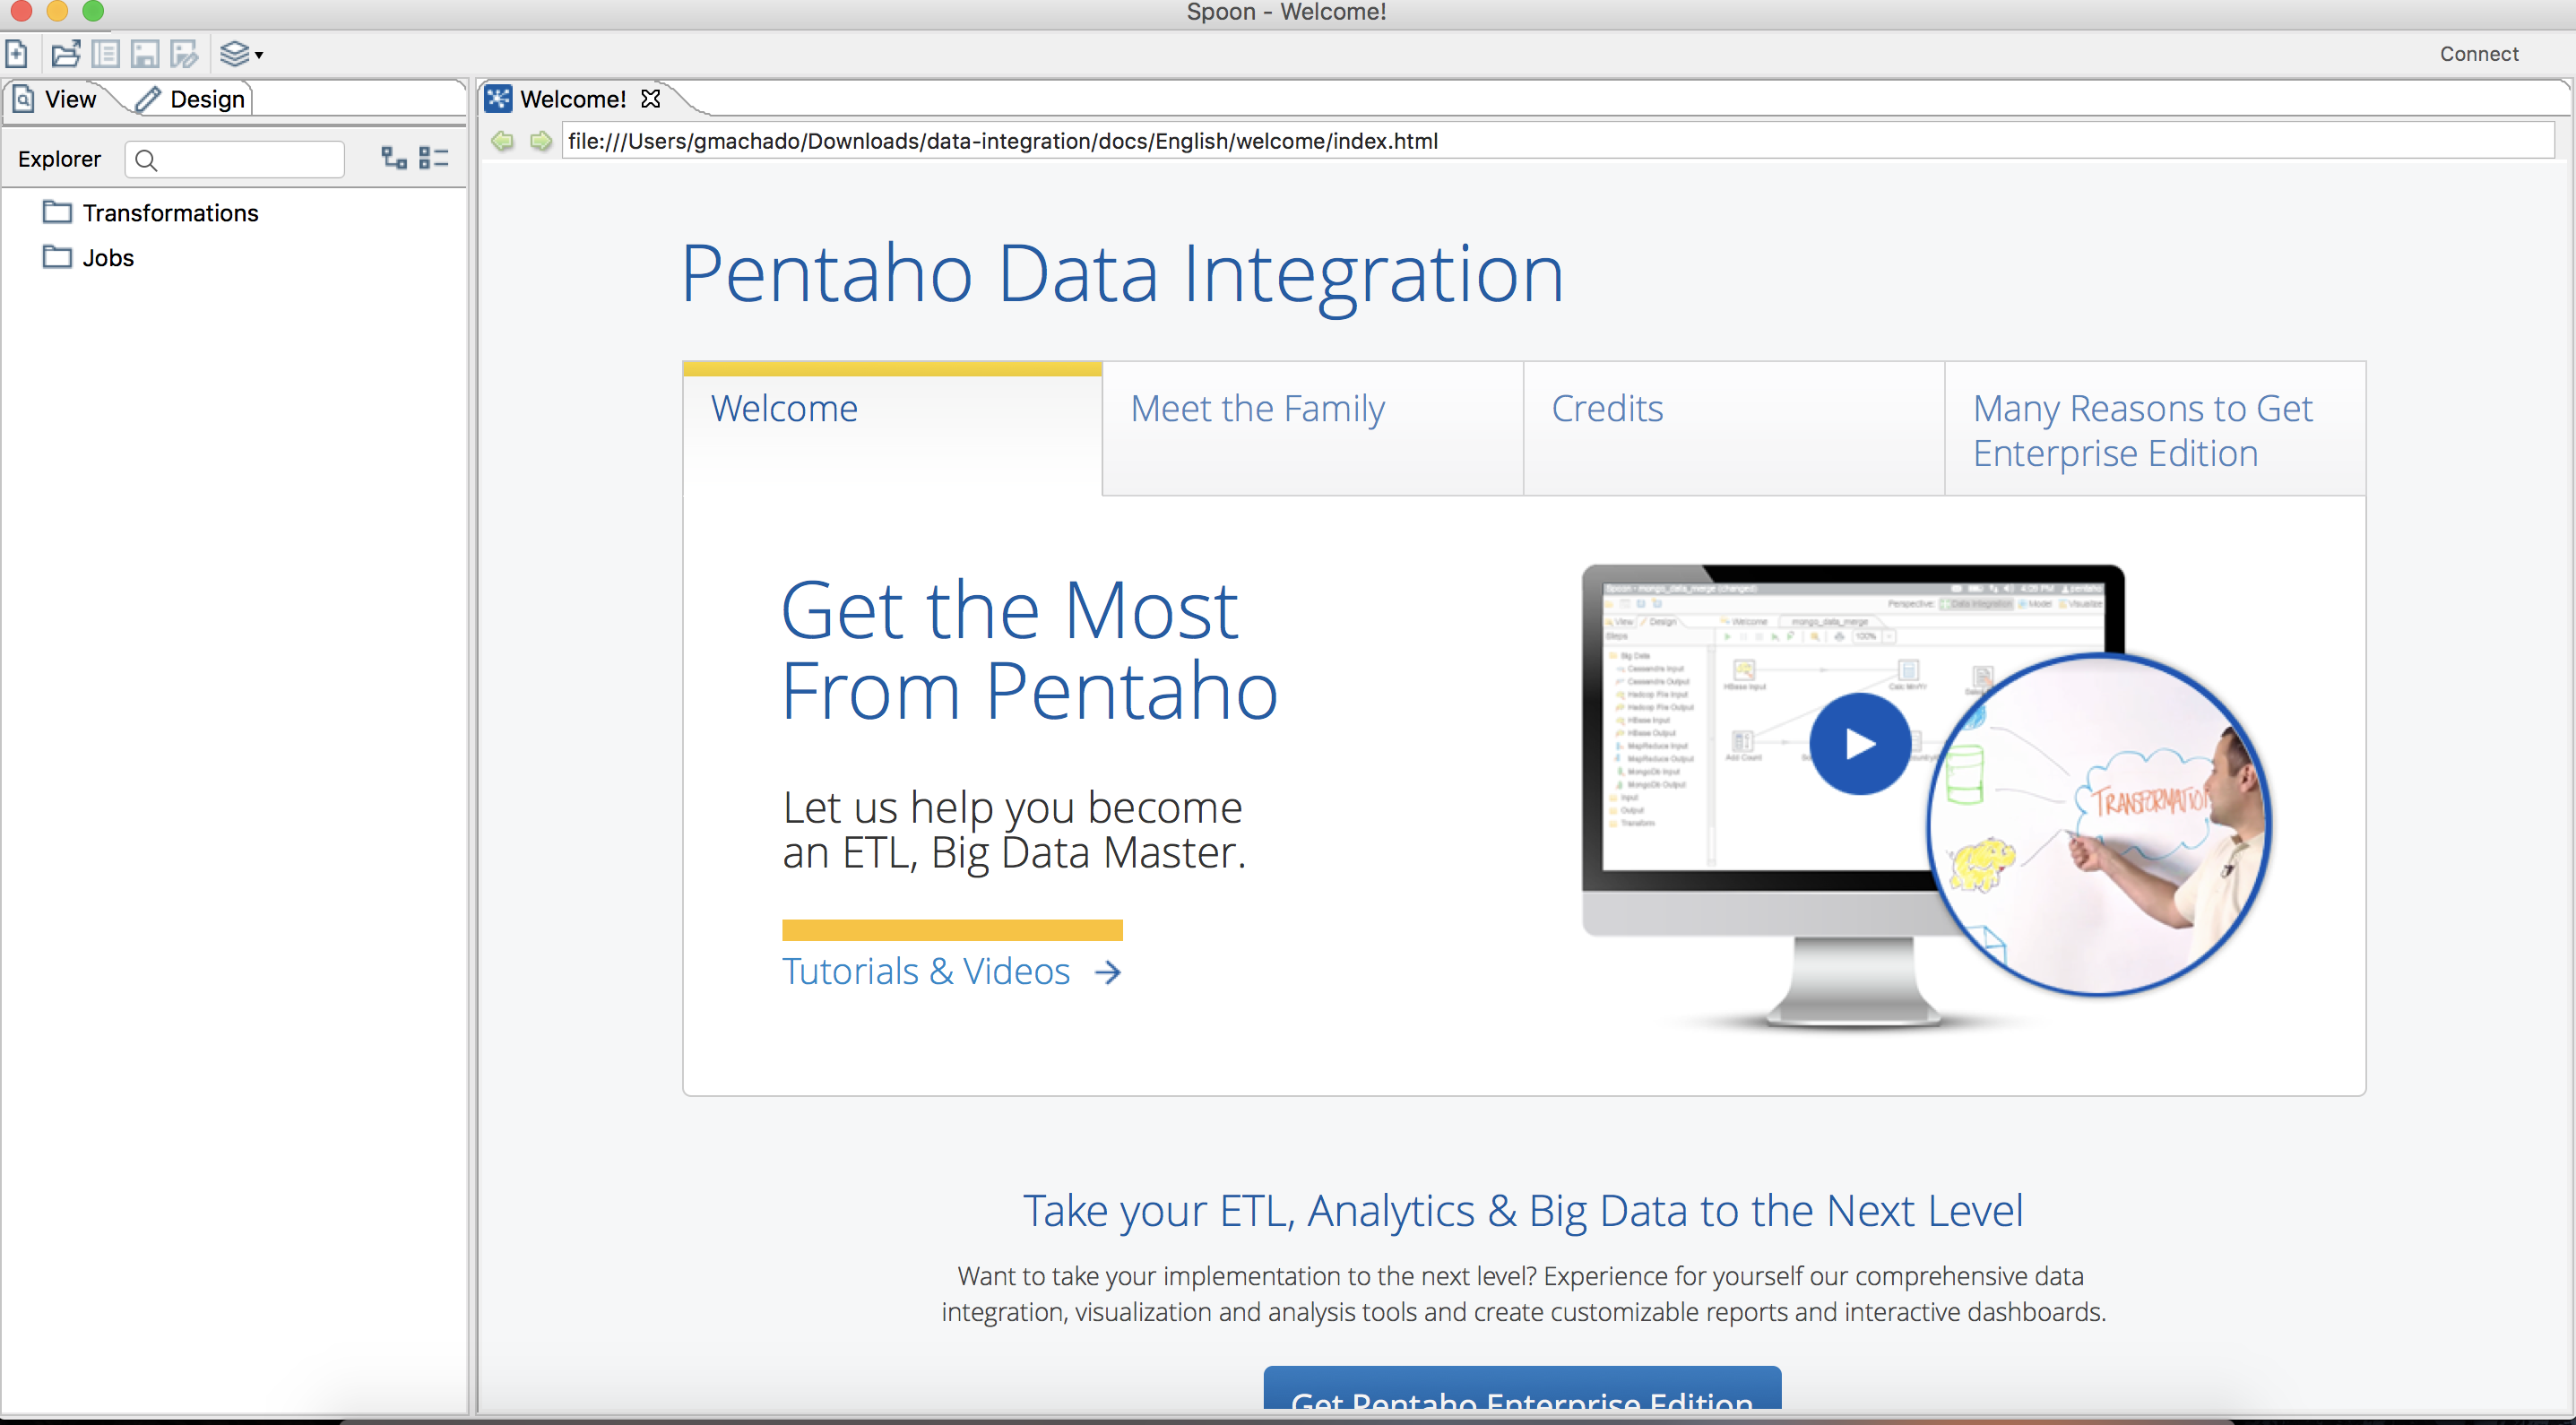
\includegraphics[height=5cm]{imagens/pagina_principal_pentaho.png}
\caption{Página inicial do \pdi}
\label{initialpdi}
\end{figure}
O \pdi utiliza \textit{transformations} que pode contém uma série de \textit{steps} e \textit{jobs} para realizar o processo de ETL. A figura \ref{transformationOptions} mostra algumas das opções para criação de transformations.
\begin{figure}[H]
\centering
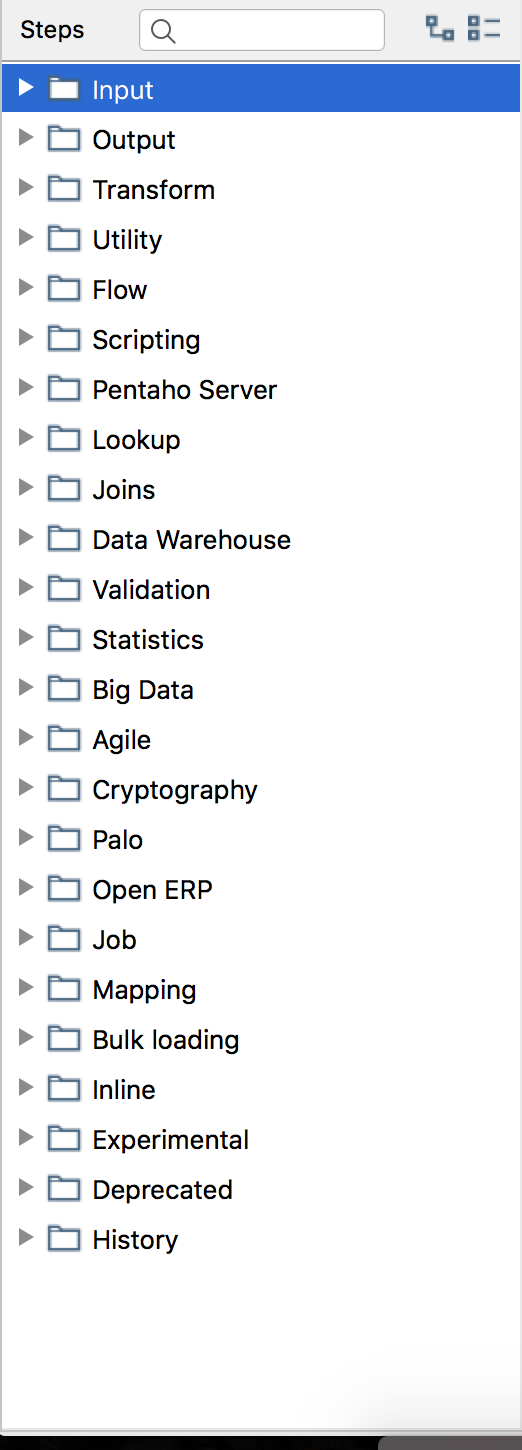
\includegraphics[width=4cm, height=8cm]{imagens/opcoes_de_transformacao.png}
\caption{Opções de transformações}
\label{transformationOptions}

\end{figure}
Transformation, segundo \citeauthor{kettle} (\citeyear{kettle}), consiste em um ou mais \textit{steps} que realiza a leitura de arquivos, filtrar linhas, limpeza dos dados e carregamento dos dados em uma base de dados. Os steps são conectados por \textit{hops}, que são caminhos de um único sentido por onde os dados trafegam. 
\begin{figure}[H]
\centering
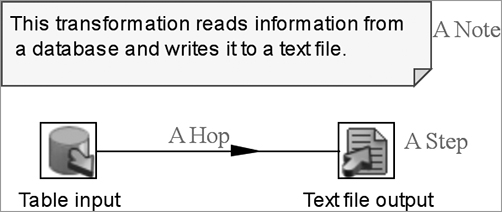
\includegraphics[height=5cm]{imagens/transformation.png}
\caption{Transformation (\citeauthor{kettle} \citeyear{kettle})}
\label{transformation}
\end{figure}

A figura \ref{transformation} mostra um pequeno exemplo pequeno de uma \textit{transformation} no \pdi.

Um \textit{step} é representado graficamente por um bloco, eles precisam ter um nome único. \citeAuthorPageYear{kettle} diz que um step é capaz de ler e de escrever linhas de dados. Os steps escrevem dados nos \textit{outcoming hops}, que são conectados a um ou mais steps no final do hop, esse hop é chamado de \textit{incomming hop} os dados são lidos nos incoming hops. Além disso, um cada step tem uma capacidade diferente, como a figura acima mostra, que o o primeiro irá receber dados de uma tabela e o segundo irá escrever os dados em um arquivo.

Um \textit{hop} é representado por uma seta ligando dois steps, que define o fluxo dos dados entre eles \citep{kettle}. Um hop também representa um buffer de dados, chamado de row set, que quando está cheio, o step que escreve os dados para e quando está vazio, o step que lê os dados aguarda até que mais dadas sejam escritos.

Os jobs são um conjunto de um ou mais \textit{jobs entries} que são executados em uma certa ordem. A figura \ref{jobsOptions} mostra algumas opções que podem ser utilizadas para criar jobs. Os job entries, assim como os steps, são passos que são executados. Eles são conectados utilizando \textit{job hops}, que definem o caminho de execução entre os job entries (\citeauthor{kettle}, \citeyear{kettle}).
\begin{figure}[H]
\centering
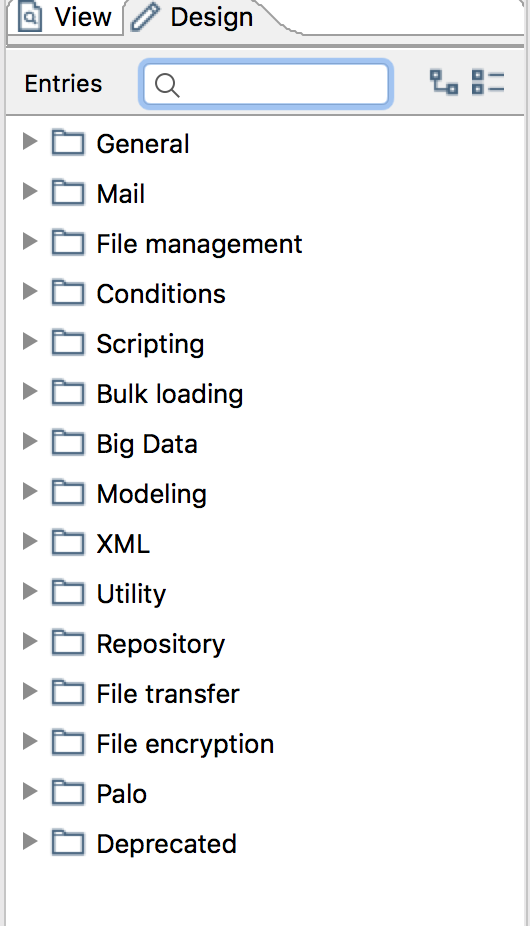
\includegraphics[width=7cm, height=9cm]{imagens/opcoes_de_jobs.png}
\caption{Opções de Jobs}
\label{jobsOptions}
\end{figure}
\subsubsection{Extract}
O \pdi oferece ferramentas para extração dos dados de fontes como arquivos de texto, planilhas, metadados, xml, banco de dados. Como mostrado na figura \ref{inputOptions}, a opção \textit{input} tem várias opções para realizar a entrada de dados. \\
\begin{figure}[H]
\centering
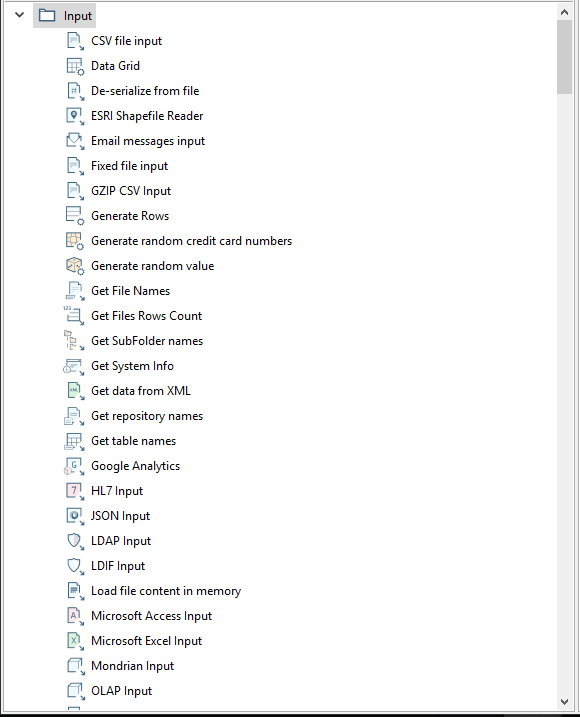
\includegraphics[width=7cm, height=9cm]{imagens/input.png}
\caption{Steps da categoria input}
\label{inputOptions}
\end{figure}
Um dos steps responsaveis pela extração é o \textit{Text file input}, que recebe um arquivo de texto, geralmente csv, e consegue fazer a extração dos campos desejados.
No exemplo abaixo, um arquivo foi carregado com as informações da tabela \ref{autores}:\\
\begin{table}[H]
\centering
\caption{ Autores }
\vspace{0.2in}
\newcolumntype{C}{>{\centering\arraybackslash}X}%
\newcommand{\rowstyle}[1]{%
  \protected\gdef\currentrowstyle{#1}%
}
\begin{tabularx}{\textwidth}{C|C|C|C|C}
\hline 
\textbf {Sobrenome} & \textbf{Nome} &\textbf{ País } & \textbf{Ano de Nascimento} &\textbf{Ano de Falecimento} \\ \hline \hline
Machado &Gabriel &Americano &1986 &2015 \\ \hline
King &Stephen &Americano &1989 &2016 \\ \hline                         
Carlos &Matheus &Brasileiro &1988 &2016 \\ \hline                       
Maria &Ana &Americana &1980 &2009 \\ \hline                         
\end{tabularx}
\label{autores}
\end{table}
Foi utilizado um step chamado \textit{Dummy} (figura \ref{dummy}) que faz absolutamente nada, apenas recebe os dados:
\begin{figure}[H]
\centering
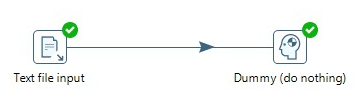
\includegraphics[height=4cm]{imagens/example1.png}
\caption{Dummy}
\label{dummy}
\end{figure}
Após a execução, as métricas de cada step podem ser observadas, a figura \ref{metrics} mostra que o step Text file input escreveu 5 registros e o Dummy leu 5.
\begin{figure}[H]
\centering
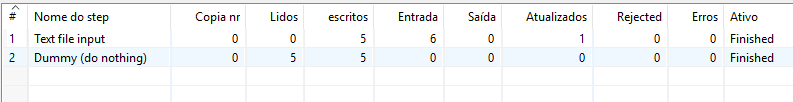
\includegraphics[height=2cm]{imagens/metrics.png}
\caption{Métricas dos steps}
\label{metrics}
\end{figure}
\vfill
\subsubsection{Transform}
Existem diversas transformações que podem ser realizadas nos dados extraídos, como limpeza de campos nulos, geração de novos atributos, formatação de campos. Para isso, o \pdi oferece diversas ferramentas para realizar esse trabalho, como mostra a figura \ref{transformsteps} abaixo.
\begin{figure}[H]
\centering
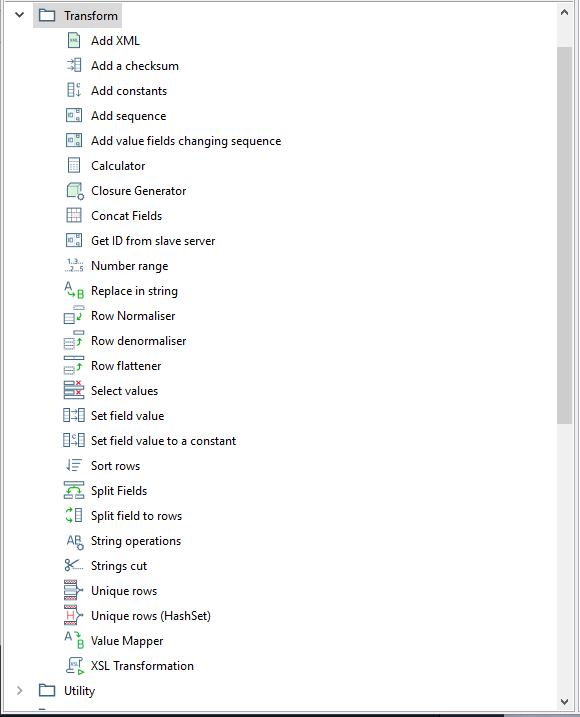
\includegraphics[width=7cm, height=9cm]{imagens/transforms.png}
\caption{Steps da categoria transform}
\label{transformsteps}
\end{figure}
Utilizando os mesmos dados da tabela anterior, novos campos podem ser adicionados, como tempo de vida. Para isso um step da aba \textit{transformation} é utilizado, o \textit{calculator} (\ref{calculator}):
\begin{figure}[H]
\centering
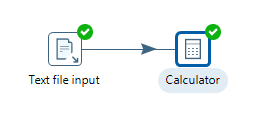
\includegraphics[height=3cm]{imagens/calc.png}
\caption{Step calculator}
\label{calculator}
\end{figure}
Esse step irá calcular o tempo de vida da pessoa utilizando o ano de nascimento e o ano de falecimento, como mostrado na figura \ref{timespan} abaixo:
\begin{figure}[H]
\centering
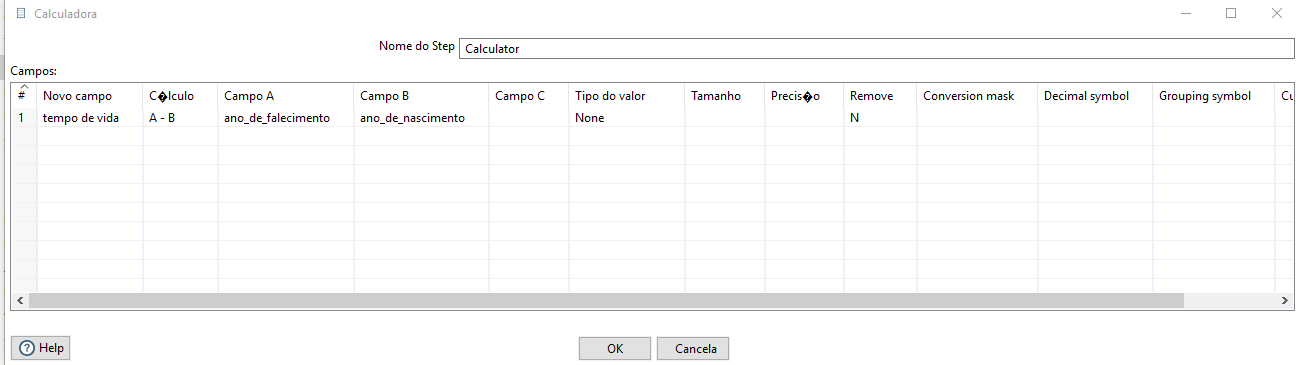
\includegraphics[height=4cm]{imagens/tempovida.png}
\caption{Cálculo do tempo de vida}
\label{timespan}
\end{figure}
A saída desse step pode ser vista no \textit{preview} (\ref{preview}):
\begin{figure}[H]
\centering
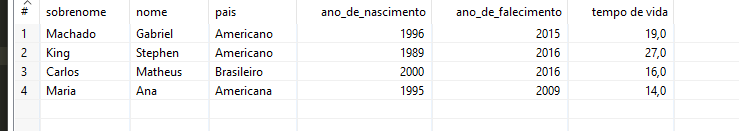
\includegraphics[height=2cm]{imagens/saidavida.png}
\caption{Saída do step}
\label{preview}
\end{figure}
\subsubsection{Load}
A ultima etapa do ETL é o Load (carregamento), o \pdi oferece diversas formas de carregamento, como mostra na figura \ref{outputsteps}.
\begin{figure}[H]
\centering
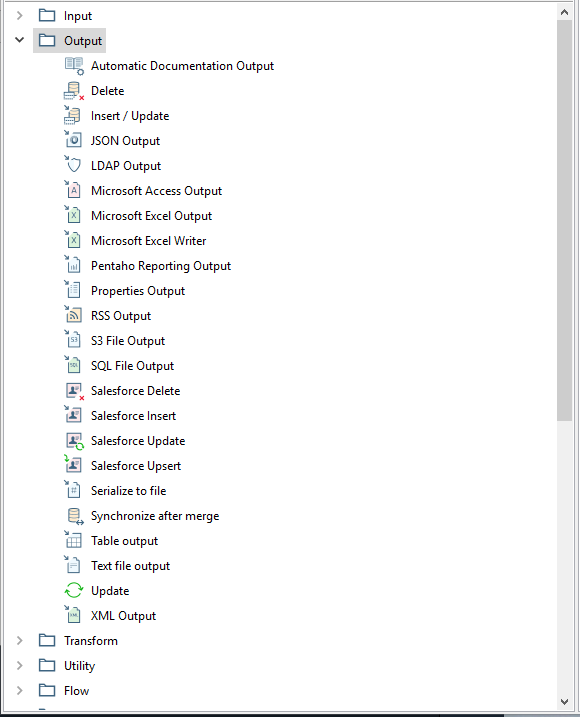
\includegraphics[width=7cm, height=9cm]{imagens/output.png}
\caption{Steps da categoria output}
\label{outputsteps}
\end{figure}
Usando os dados gerados na etapa de transformação, os dados serão carregados em uma tabela no banco de dados, para isso é necessário definir uma conexão no Pentaho e usar o step \textit{Table output}, como mostra a figura \ref{outputstep} abaixo.
\begin{figure}[H]
\centering
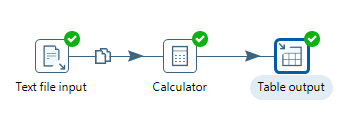
\includegraphics[height=2cm]{imagens/tableoutput.png}
\caption{Saída no banco de dados}
\label{outputstep}
\end{figure}
Na aba \textit{view}, na figura \ref{database}, existe uma opção \textit{connections} e lá tem como criar uma conexão com a base de dados escolhida, nesse caso é o postgres.\\
\begin{figure}[H]
\centering
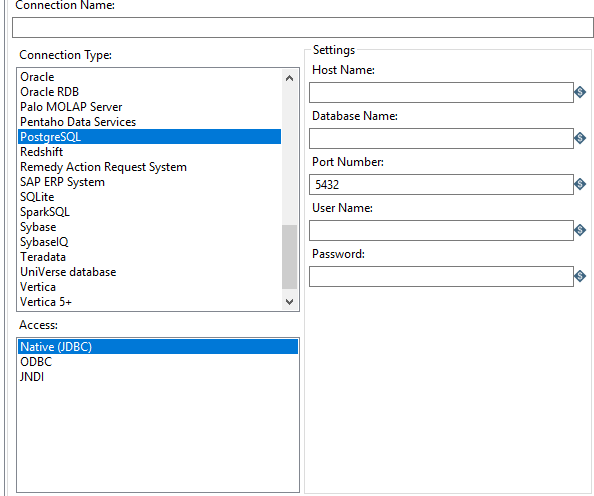
\includegraphics[height=7cm]{imagens/conexao.png}
\caption{Conexões disponíveis no \pdi}
\label{database}
\end{figure}
Quando a conexão for definida, é necessário criar utilizar o step table output (figura \ref{outputtable}), realizando o mapeamento adequado dos campos para serem inseridos na tabela.
\begin{figure}[H]
\centering
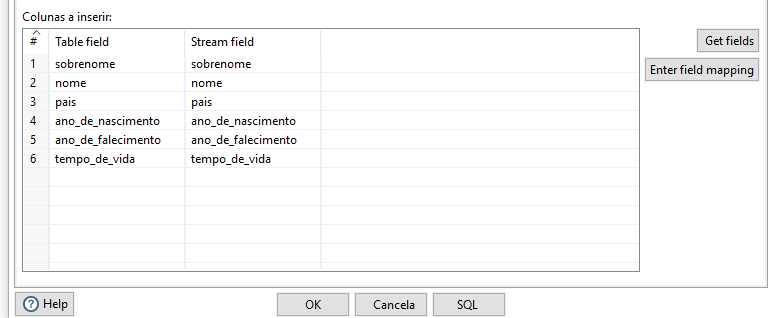
\includegraphics[height=3cm]{imagens/tablemapping.png}
\caption{Mapeamento entre os campos gerados e os campos da tabela}
\label{outputtable}
\end{figure}
Ao executar a transformação, os dados serão carregados na tabela, como mostra a figura \ref{table}.
\begin{figure}[H]
\centering
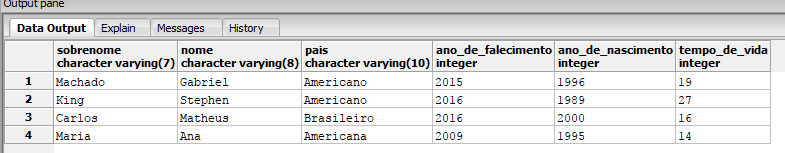
\includegraphics[height=2.5cm]{imagens/saidasql.png}
\caption{Saída no banco de dados}
\label{table}
\end{figure}

\section{Mineração de Dados}

\citeAuthorPageYear{jmj} dizem que o termo mineração de dados poderia ter sido chamado de mineração de conhecimentos dos dados, já que minerar é um processo para encontrar pequenas quantidades de preciosidades de uma grande quantidade de material bruto. 

Outros podem falar que mineração de dados é um sinônimo de KDD (knowledge discovery from data), descobrimento de conhecimento a partir de dados. A mineração também pode ser vista como um passo essencial no processo de descoberta de conhecimento, como mostra a figura \ref{kdd}. 

\begin{figure}[H]
\centering
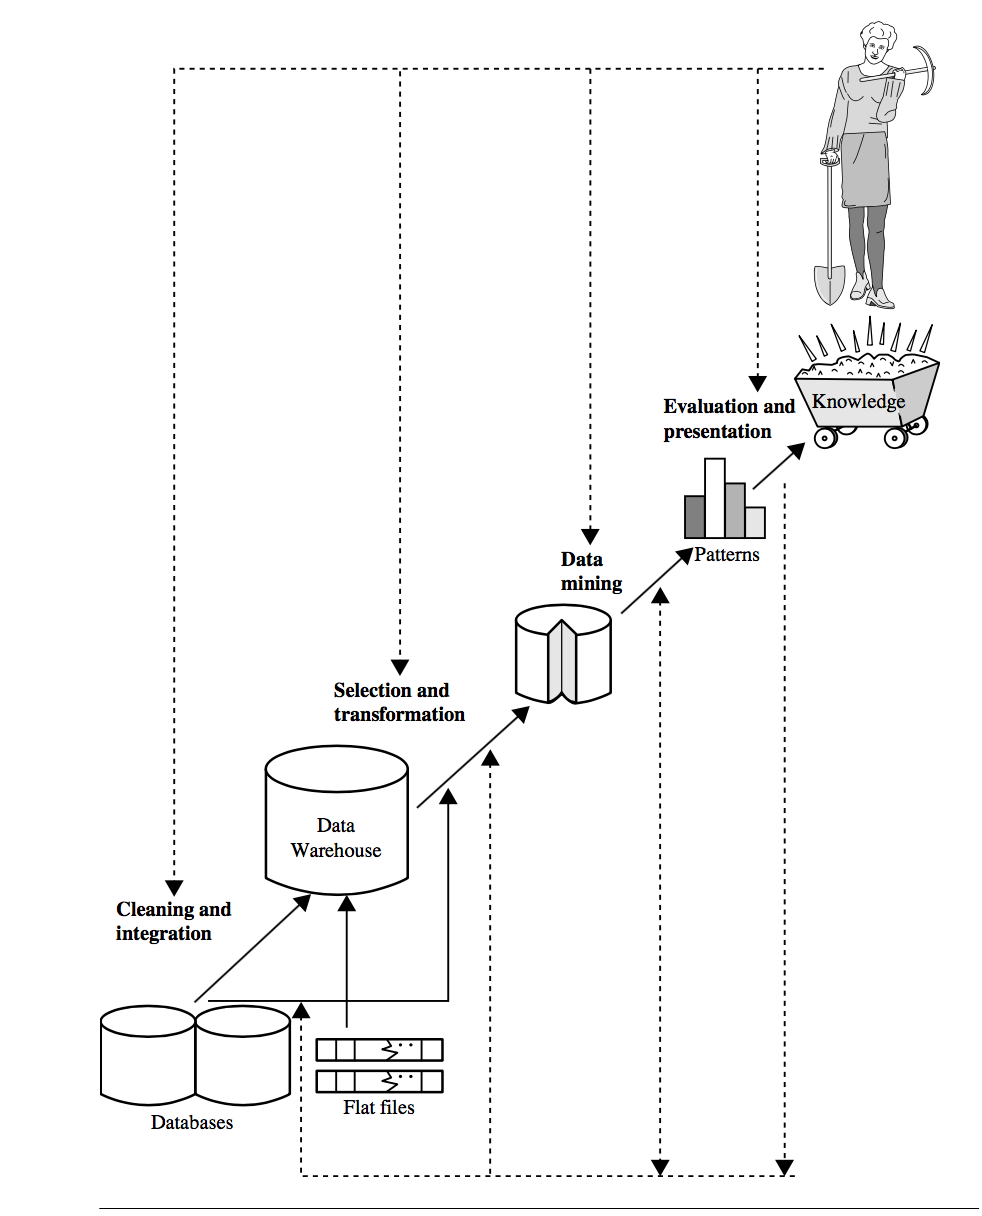
\includegraphics[height=9cm, width=9cm]{imagens/kdd.png}
\caption{Mineração de dados como um processo de descoberta de conhecimento \citep{jmj}}
\label{kdd}
\end{figure}

\citeauthor{jmj} sumarizam mineração de dados em o processo de descobrir padrões interessantes e conhecimento a partir de grandes quantidades de dados. Essas fontes podem ser banco de dados, a internet, data warehouses, dados transacionais, stream de dados, arquivos e etc. 

A mineração de dados tem diversas funcionalidades, como caracterização, que é a sumarização das características gerais de uma classe alvo de dados, discriminação, que é a comparação das características gerais de uma classe alvo com as características de uma ou mais classes diferentes \citep{jmj}. 

Também é usada para encontrar padrões que aparecem frequentemente nos dados. Existem alguns tipos de padrões, como \textit{frequent itemset}, que são itens que geralmente aparecem juntos em um conjunto de dados transacionais, \textit{frequent subsequence} ou \textit{sequencial pattern}, que pode ser o padrão de um cliente que compra primeiro um notebook, depois uma câmera digital e depois um cartão de memória \citep{jmj}. Por último, tem as \textit{frequent substructures}, que, segundo \citeauthor{jmj}, são formas estruturadas que podem aparecer frequentemente, como grafos e árvores, que podem conter \textit{itemsets} e \textit{subsequences}.

Algoritmos de classificação e regressão podem ser usados para analises preditivas, tentando prever dados categóricos ou discretos. A classificação, é o processo de encontrar um modelo que melhor expressa uma classe, esse modelo é derivado da analise de um conjunto de treinamento \citep{jmj}. Os modelos podem ser representados usando árvores de decisão, formulas matemáticas, redes neurais e etc.

Já a regressão, o uso mais comum é para tentar prever valores numéricos contínuos, utilizando algoritmos como regressão linear, regressão lasso e etc.

Também existem os algoritmos de clusterização, que, diferente da classificação e regressão, esse processo analisa os dados sem consultar as suas classes \citep{jmj}. Em alguns casos, os dados podem até vir sem classe. \citeauthor{jmj} diz que a clusterização pode ser usada para encontrar classes para os grupos de dados. Os clusters são formados de uma forma que os objetos dentro deles tenham uma grande similaridade ao se compararem, mas bem diferentes dos objetos em outros clusters \citep{jmj}.

\subsection{CRISP-DM}
\subsubsection{O que é CRISP-DM}
CRISP-DM, ou Cross-industry standard process for data mining, é uma técnica utilizada no processo de mineração de dados, com uma série de tarefas a serem realizadas para chegar ao melhor resultado.
Segundo \citeauthor{dmfd} (\citeyear{dmfd}), mineração de dados não é algo feito uma vez e depois esquecido, o trabalho pode ser aplicado em outros projetos, pode servir de referência
O ciclo de vida da mineração de dados contém seis fases, como apresentado na figura \ref{crispcycle}: entendimento do negócio, entendimento dos dados, preparação dos dados, modelagem, avaliação e implementação. 
A mineração de dados não termina uma vez que a solução é implementada \citep{crispmanual}
\begin{figure}[H]
\centering
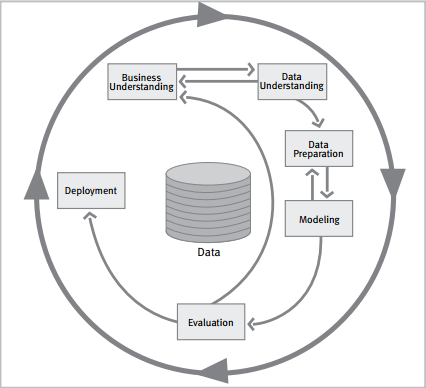
\includegraphics[height=6.2cm]{imagens/lifecycle.png}
\caption{Ciclo de vida (\citeauthor{crispmanual} \citeyear{crispmanual})}
\label{crispcycle}
\end{figure}
Cada uma dessas fases tem diversas tarefas que são realizadas para completar cada uma das fases e cada tarefa tem suas saídas.
\subsubsection{Entendimento do negócio}
A primeira fase do CRISP-DM é o entendimento do negócio, que foca em entender os objetivos do negócio e seus requerimentos de uma perspectiva de negócio.

O primeiro objetivo da analise de dados é entender, sob uma perspectiva de negócio, o que o cliente deseja realizar. Segundo \citeauthor{dmfd} (\citeyear{dmfd}), deve ter um entendimento claro do problema que deseja abordar, o objetivo do negócio, as limitações e o impacto. Esse processo produz uma informação da situação do negócio, objetivo do cliente e o critério de sucesso.

Depois é realizada uma avaliação da situação, essa tarefa consiste em um detalhamento maior dos recursos, limitações, premissas e outros fatores que devem ser considerados ao determinar os objetivos da análise de dados e do plano de projeto \citep[p. 14]{crispmanual}.

Outra etapa é determinar os objetivos da mineração de dados, por exemplo, como "prever quantas pessoas irão visitar uma loja no verão, de acordo com informações dos últimos 2 anos dessa loja".

E então é necessário produzir plano de projeto Descrever o plano desejado para atingir os objetivos da mineração de dados e desse modo, os objetivos do negócio \citep{crispmanual}. Esse processo produz o plano de projeto e avaliações iniciais de ferramentas e técnicas

\subsubsection{Entendimento dos dados}
Segundo \citeauthor{dmfd} (\citeyear{dmfd}), na segunda fase do projeto de mineração de dados, os dados tem que ser obtidos e tem que verificar se eles são apropriados para as necessidades.

A primeira tarefa dessa fase é coletar dados iniciais e então realizar, caso necessário, o carregamento dos dados em alguma ferramenta. Nessa tarefa é produzida uma lista de todos os datasets adquiridos, junto com localizações, métodos utilizados para coleta e problemas encontrados.

Depois, é feito a descrição dos dados, exploração usando técnicas de visualização. Essa análise pode estar diretamente ligada aos objetivos da mineração de dados \citep{crispmanual}. Essa tarefa produz um relatório da exploração de dados, contendo descobertas iniciais ou hipóteses, e o seu impacto no restante do projeto \citep{crispmanual}.

Depois, é necessário verificar a qualidade dos dados, respondendo perguntas como "os dados estão completos?", "existem valores faltantes?". É criado um relatório da qualidade de dados, com uma lista de problemas encontrados e suas soluções.

\subsubsection{Preparação dos Dados}
A maior parte do tempo gasto no processo de mineração de dados é na preparação deles, já que diversos tratamentos precisam ser feitos nos dados e isso nem sempre é tão simples. A maior parte dos dados usados para mineração foram originalmente coletados e preservados para outros objetivos e precisa ser refinado antes de ser ficar pronto para a modelagem \citep{dmfd}.

Essa fase tem duas saídas, antes das tarefas, que são: \textbf{datasets}, que são os dados produzidos nessa fase e serão usados para modelagem e \textbf{descrição do dataset} \citep{crispmanual}.

A primeira tarefa é \textbf{selecionar os dados} que serão usados na modelagem, baseado nos objetivos da mineração de dados, qualidade e limites técnicos \citep{crispmanual}. É criada uma lista de dados que foram incluídos e excluídos e a razão para isso.

Depois é feita uma \textbf{limpeza dos dados}, que eleva a qualidade dos dados para o nível requerido pelas técnicas de analise selecionadas \citep{crispmanual}. Segundo \citeauthor{dmfd} (\citeyear{dmfd}), dificilmente os dados selecionados estarão perfeitamente limpos, mudanças precisarão ser feitas nos dados para atingir o nível necessário. \citeauthor{crispmanual} (\citeyear{crispmanual}) diz que transformações nos dados podem ser feitas para limpeza e possível impacto na análise de resultados. Nessa etapa é criado um relatório de limpeza de dados: que descreve as ações tomadas para lidar com os problemas encontrados anteriormente.

A tarefa seguinte é \textbf{Construir dados}, essa tarefa consiste na criação de novos campos, dados agregados, ou novos formatos de dados. É produzida uma lista de atributos criados a partir dos atributos existentes e explicar como e por que eles foram criados e uma lista de registros criados, junto com o motivo e como eles foram criados.

A próxima tarefa é \textbf{integrar dados}, já que eles podem estar em diferentes datasets e é necessário a integração desses dados para a fase de modelagem.A saída dessa fase é: \textbf{dados fundidos}: fundir tabelas se refere a juntar duas ou mais tabelas que tem diferentes informações sobre o mesmo objeto \citep{crispmanual}. 

Por último, é necessário \textbf{formatar dados}. Dados frequentemente vem em formatos que não são os convencionais para modelagem \citep{dmfd}, então conversões precisam ser feitas. \citeauthor{dmfd} (\citeyear{dmfd}) afirma que a fase de preparação de dados deve ser finalizada com um dataset pronto para modelagem e um relatório descrevendo o dataset.

A saída é dados reformatados, convertidos para alguma unidade de medida única para todos os dados (como quilos, em peso).

\subsubsection{Modelagem}
É a fase onde alguma técnica de aprendizado de máquina é utilizada, testada e avaliada para encontrar padrões nos dados, como K-nearest neighbors, Decision Tree e etc.

O primeiro passo da modelagem é \textbf{selecionar a técnica de modelagem} que será usada, caso múltiplas técnicas sejam aplicadas, é necessário executar essa tarefa para cada uma delas \citep{crispmanual}. Nem todas as técnicas de modelagem serão uteis para as necessidades do negócio.

Depois é necessário \textbf{gerar o teste de design}, ou seja gerar procedimentos ou mecanismos para testar a qualidade e validade do modelo \citep{crispmanual}. Os dados geralmente são separados em dois conjuntos, o conjunto de treinamento e o conjunto de teste. O conjunto de treinamento é usado para construir o modelo e o de teste para validar ele. Nessa etapa é gerado descrito como planeja, treina, testa e avalia o modelo.

Depois, é a fase de \textbf{construir o modelo}, Rodar a ferramenta de modelagem para criar um ou mais modelos \citep{crispmanual}. Esse processo produz um documento com as configurações de parâmetros usados, modelos produzidos pela ferramenta e uma descrição dos modelos.

Por fim, é a fase de \textbf{avaliar o modelo}, que sumariza os dados e ranqueia os modelos utilizados e também revisa as configurações dos parâmetros utilizados para tentar reajusta-los até encontrar a melhor possível.

\subsubsection{Avaliação}
Avaliar todo o processo, não só os modelos mas também o processo utilizado para a sua criação.

A primeira tarefa é \textbf{avaliar resultados}. Essa tarefa avalia o grau em que o modelo se adequa ao objetivo original do negócio e busca determinar se existe alguma razão para o modelo estar deficiente.

Essa tarefa avalia o resultado da mineração de dados a respeito do critério de sucesso do negócio (\citeauthor{dmfd} (\citeyear{dmfd}) afirma que essa tarefa serve para dizer se o projeto atingiu ou não os objetivos definidos no início e seleciona os modelos que atingiram o critério selecionado.

Depois é feita uma \textbf{revisão do processo}, nesse ponto, os modelos resultantes aparentam ser satisfatórios para a necessidade do negócio \citep{crispmanual}. Essa é uma fase usada para rever o processo, como algum problema que foi negligenciado. \citeauthor{crispmanual} (\citeyear{crispmanual}) diz que se deve sumarizar a revisão e ressaltar as atividades que não foram realizadas e aquelas que devem ser repetidas.

A última fase é \textbf{determinar próximos passos}. A fase de avaliação é concluída com as recomendações para o próximo passo \citep{dmfd}. Decidir se deve finalizar o projeto ou continuar o desenvolvimento. Essa fase também inclui a análise das despesas  e recursos restantes, que podem influenciar na decisão \citep{crispmanual}.
Essa fase produz uma lista de possíveis ações e a decisão.


\subsubsection{Implementação}
O objetivo dessa fase final é a implementação do modelo.
A primeira fase é o plano de implementação, essa fase usa os resultados da avaliação e determina a estratégia de implementação \citep{crispmanual}. 

Ela produz um plano de implementação que sumarizar as estratégias para implementação, os passos necessários e como realizar.
Depois é feito um \textbf{Plano de monitoramento e manutenção}, segundo \citeauthor{dmfd} (\citeyear{dmfd}), mineração de dados é um ciclo, então é necessário continuar envolvido com os modelos enquanto eles são integrados ao dia-a-dia. A preparação cuidadosa das estratégias de manutenção ajuda a evitar longos períodos desnecessários de uso incorreto dos resultados da mineração \citep{crispmanual}.

Ela produz um plano de monitoramento e manutenção que sumarizar todas as estratégias de manutenção e monitoramento, incluindo os passos necessários para realiza-los \citep{crispmanual}.
Em seguida, é feito um \textbf{Relatório Final}, que pode ser somente um sumário do projeto e das experiências ou uma apresentação final e compreensível dos resultados da mineração \citep{crispmanual}.
Essa fase produzo relatório final, que sumariza todo o projeto ao juntar todos os relatórios criados até o momento \citep{dmfd} e apresentação final encontro realizado na conclusão do projeto com seu cliente.

Por último, é feita uma \textbf{revisão do projeto} onde o time se reúne e discute o que deu certo e o que não deu, o que pode ser feito novamente e o que não pode e o que deve ser evitado \citep{dmfd}.
A saída é uma documentação de experiência que sumarizar a experiência ganha com o projeto, como erros e acertos, dicas de como selecionar os melhores modelos para situações semelhantes e etc.

\subsection{WEKA}

O WEKA, Waikato Environment for Knowledge Analysis, é uma coleção de algoritmos de aprendizado de máquina e de ferramentas de preprocessamento de dados\citeAuthorPageYear{weka}. Ele é criado de uma forma que os algoritmos possam ser testados rapidamente nos datasets, ele também contém suporte de mineração de dados, como preparação dos dados, avaliar modelos estatisticamente, visualização dos dados e resultados da aprendizagem. Todas essas ferramentas podem ser acessadas por uma interface simples. O WEKA é escrito em Java e é distribuído sob a GNU General Public License, ele roda em quase toda plataforma e já foi testado nos sistemas operacionnais Linux, Windows e Macintosh \citeAuthorPageYear{weka}.

\citeAuthorPageYear{weka} diz que o WEKA contém métodos os principais problemas de mineração de dados, como regressão, clusterização, mineração de regras de associação e seleção de atributos. Conhecer os dados é uma parte integral do trabalho. Uma das formas de utilizar o WEKA é aplicando um método aos dados e analisar a saída para aprender mais sobre os dados \citeAuthorPageYear{weka}, outra é utilizando modelos para gerar previsões em novas instancias. Uma terceira forma é aplicar diferentes algoritmos e comparar as performances para poder selecionar um para previsão \citeAuthorPageYear{weka}. Uma terceira forma é usar diferenntes algoritmos de aprendizado e comparar seus resultados para selecionar um para fazer a previsão. \citeAuthorPageYear{weka} diz que a implementação de algoritmos de aprendizado é um dos recursos mais valiosos que o WEKA fornece, enquanto os métodos de preprocessamento, também chamados de \textit{filters}, vem logo em seguida. 

\citeAuthorPageYear{weka} diz que o WEKA pode ser facilmente usado através de uma interface gráfica chamada de \textit{Explorer}. Por exemplo, um dataset pode ser facilmente carregado e construir uma árvore de decisão em cima dele. O WEKA também tem outras interfaces, como o \textit{Knowledge Flow}, que permite processar dados via streaming e o \textit{Experimenter}, que permite responder uma pergunta bem básica e pratica: quais métodos e valores de parâmetros funcionam melhor para determinado problema? O WEKA pode fornecer um ambiente que permite usuários do WEKA comparar uma variedade de algoritmos de aprendizado. \citeAuthorPageYear{weka} diz que é possível fazer isso interativamente usando a  interface Explorer, mas o Experimenter permite automatizar o processo deixando mais fácil de de rodar classificadores e filtros em um dataset, para coletar estatísticas de performance.

Além disso, todas essas opções podem ser acessadas através de uma interface de linha de comando.

\subsection{Explorer}
A interface gráfica principal do WEKA é a Explorer. Diversas operações podem ser feitas nessa interface.

\subsubsection{Carregando os dados}
Ao abrir o WEKA, deve se selecionar a opção explorer, como mostra na figura \ref{explorer}:

\begin{figure}[H]
\centering
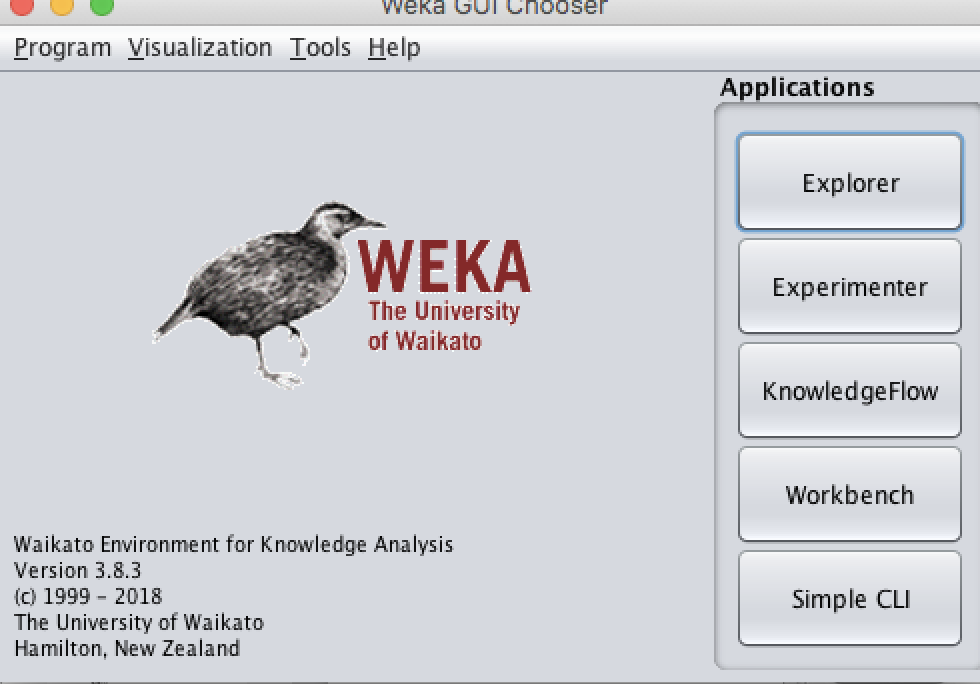
\includegraphics[height=5cm]{imagens/wekaprincipal.png}
\caption{Interface principal do WEKA}
\label{explorer}
\end{figure}

Ao abrir o explorer, a tela deverá exibir diversas opções para carregamento de dados. O formato principal do WEKA é o ARFF, porém ele também é capaz de ler outros formatos, como csv.

\begin{figure}[H]
\centering
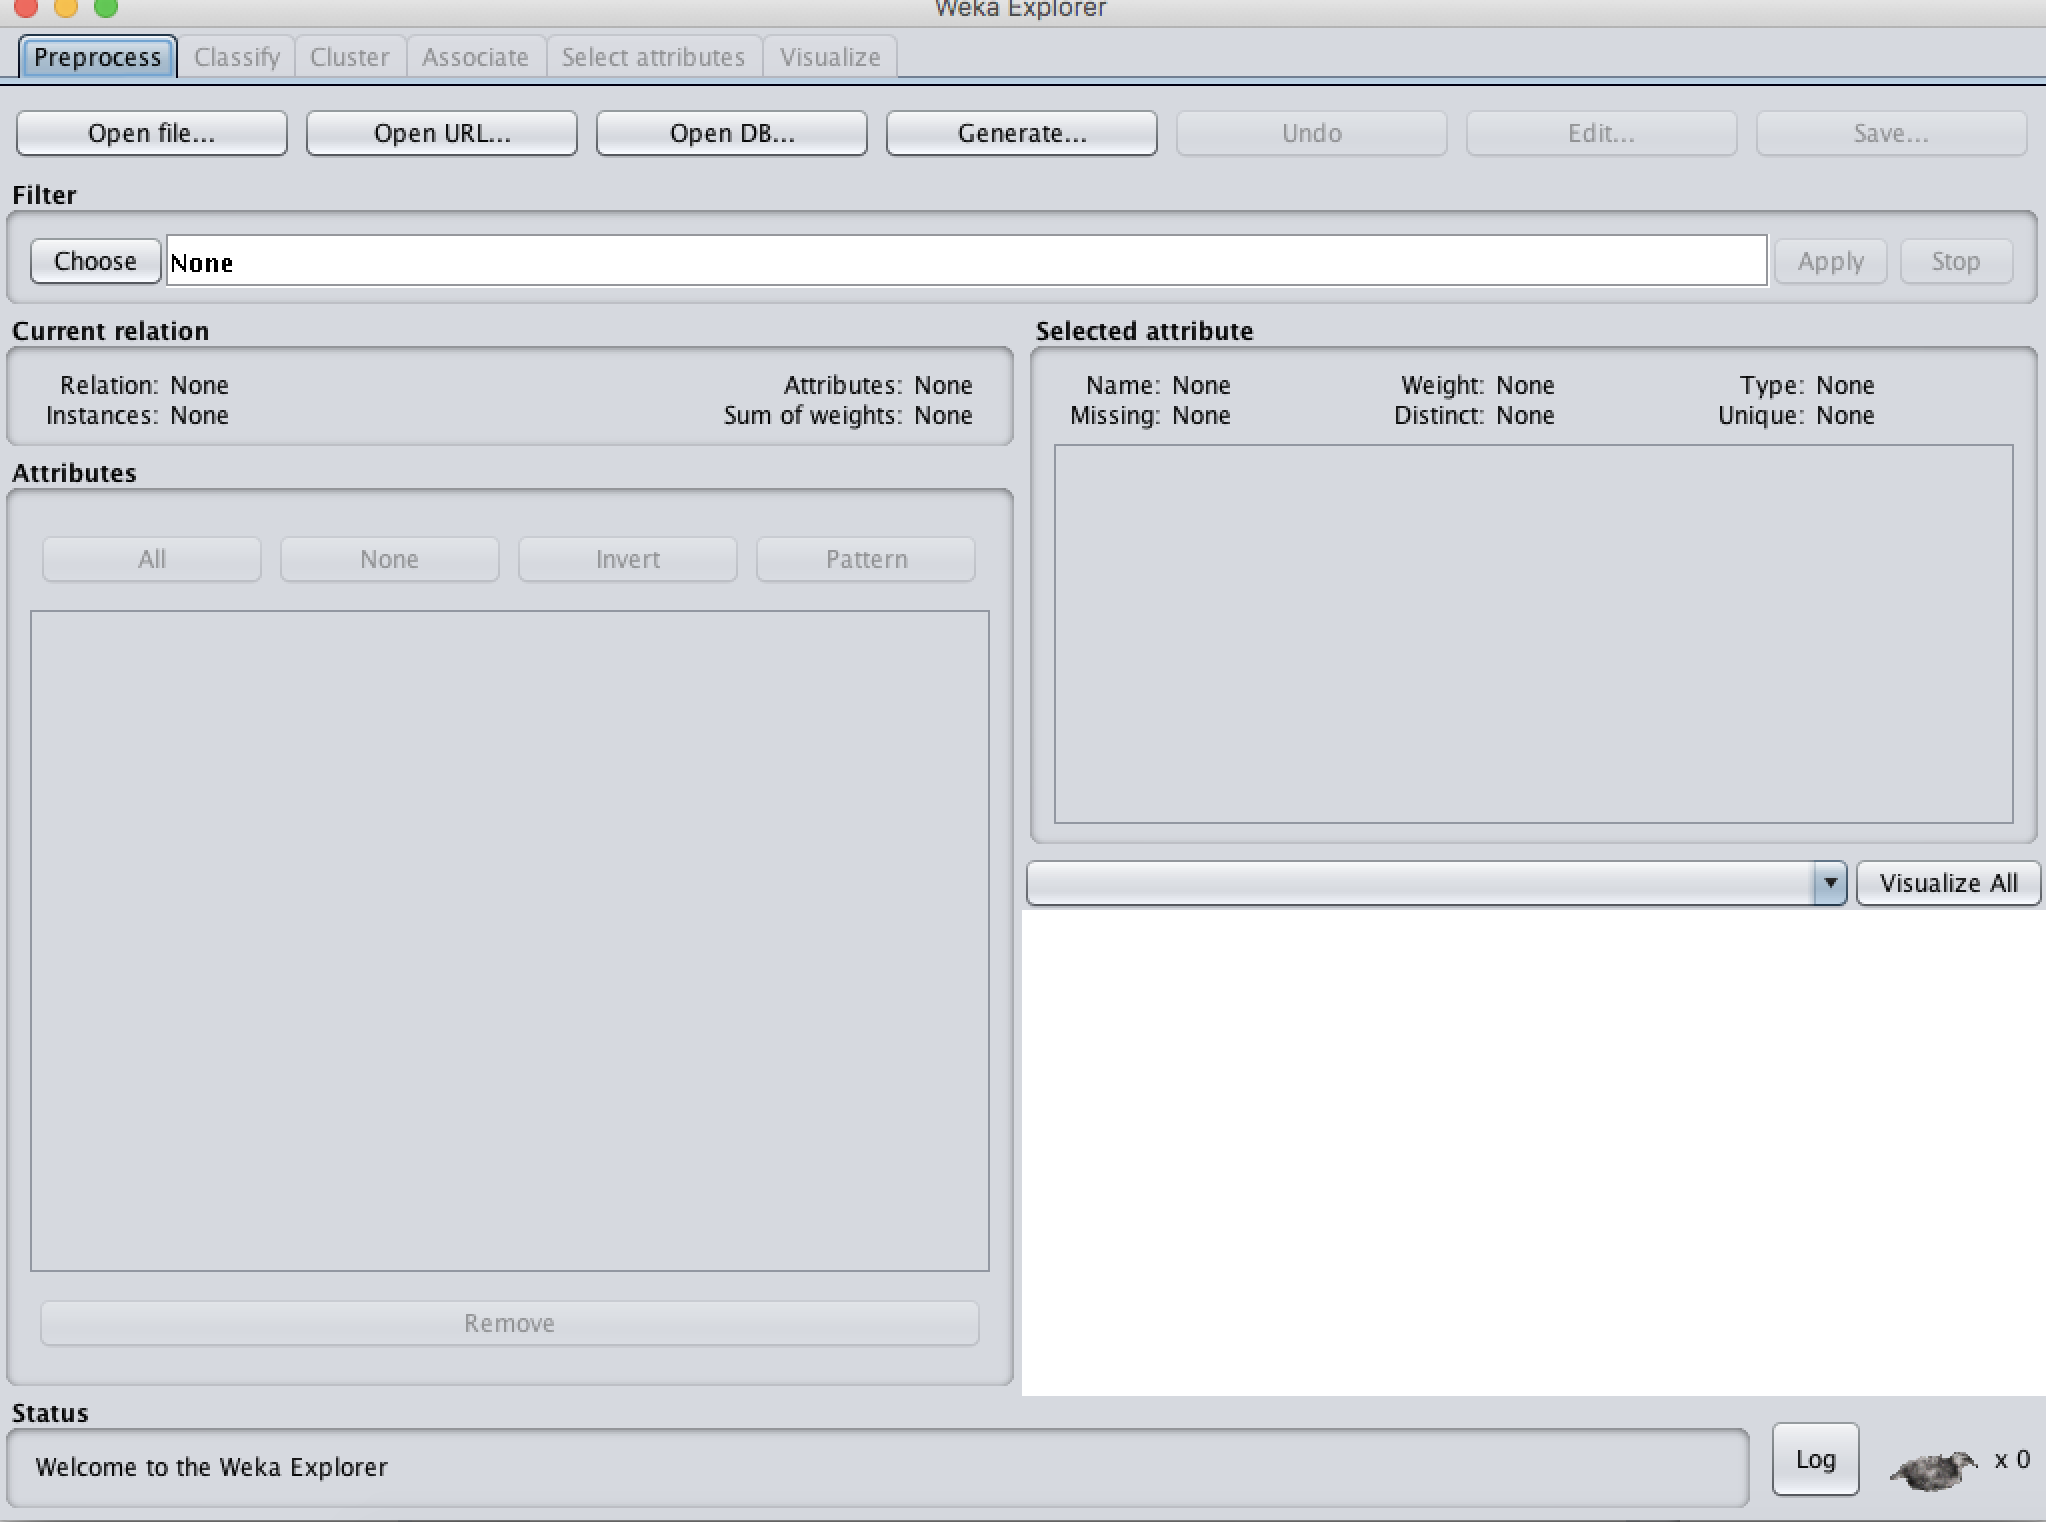
\includegraphics[height=7cm]{imagens/wekapreprocessempty.png}
\caption{Tela de preprocessamento}
\label{figura19}
\end{figure}

Ao carregar os dados, informações sobre cada um dos atributos pode ser encontrada no canto inferior direito e todos os atributos estarão listados no canto esquerdo, como mostra a figura \ref{loadeddata}. A figura \ref{distribuicao} mostra que é possível obter uma distribuição dos valores de cada um dos atributos disponíveis.

\begin{figure}[H]
\centering
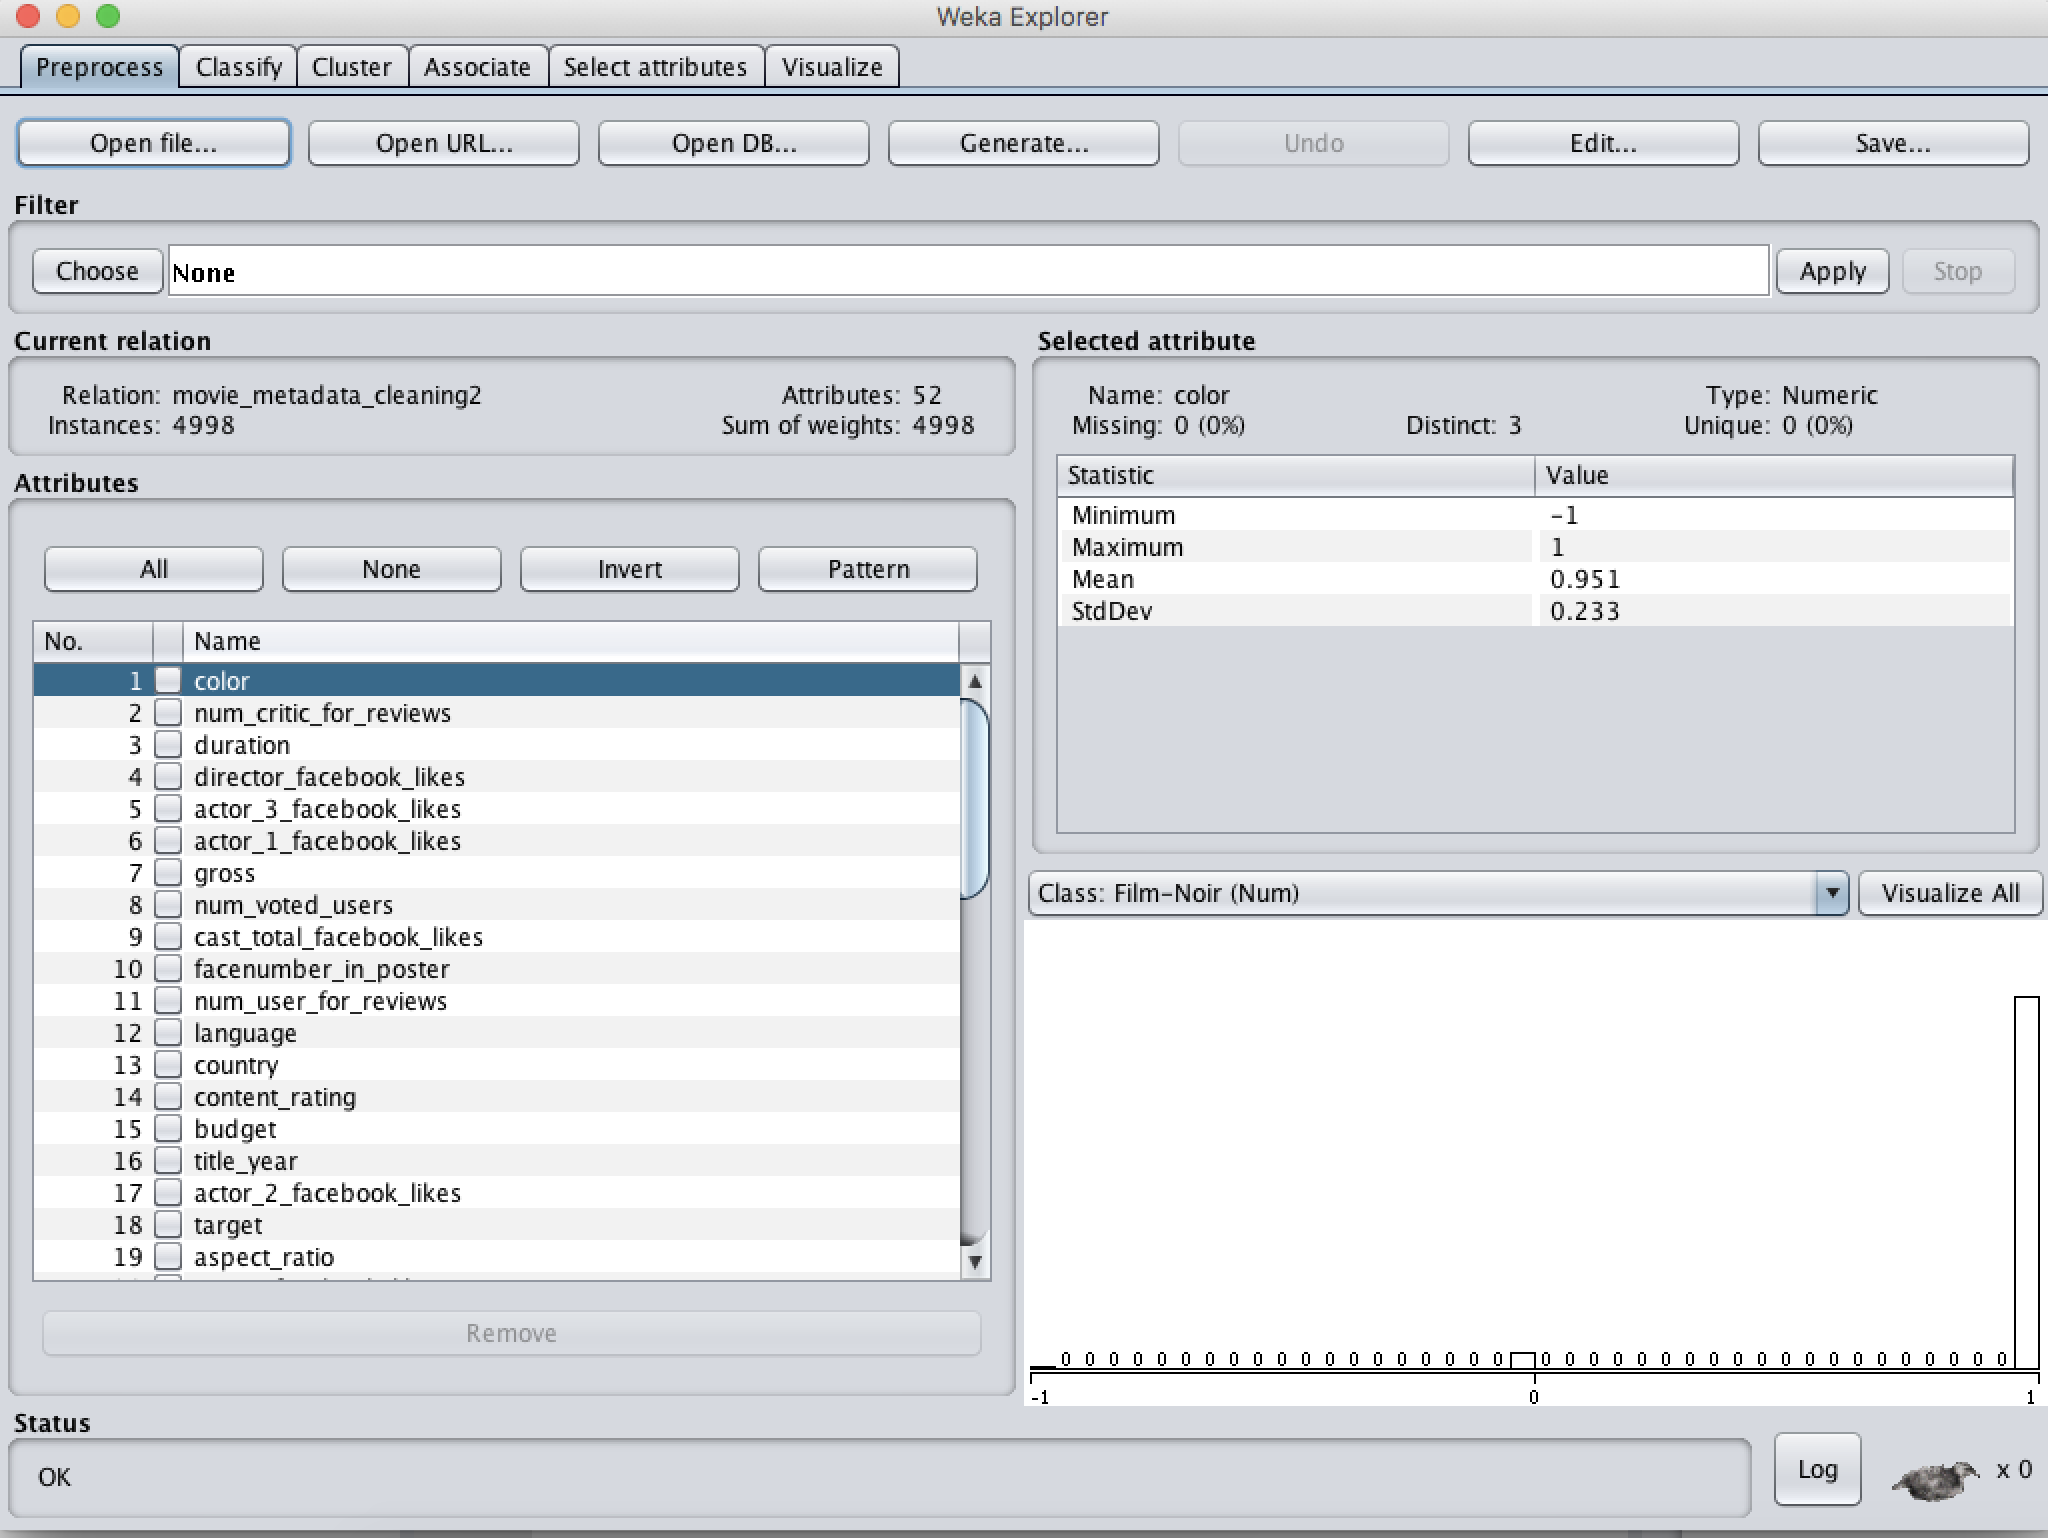
\includegraphics[height=7cm]{imagens/wekapreprocessingfull.png}
\caption{Dados carregados}
\label{loadeddata}
\end{figure}

\begin{figure}[H]
\centering
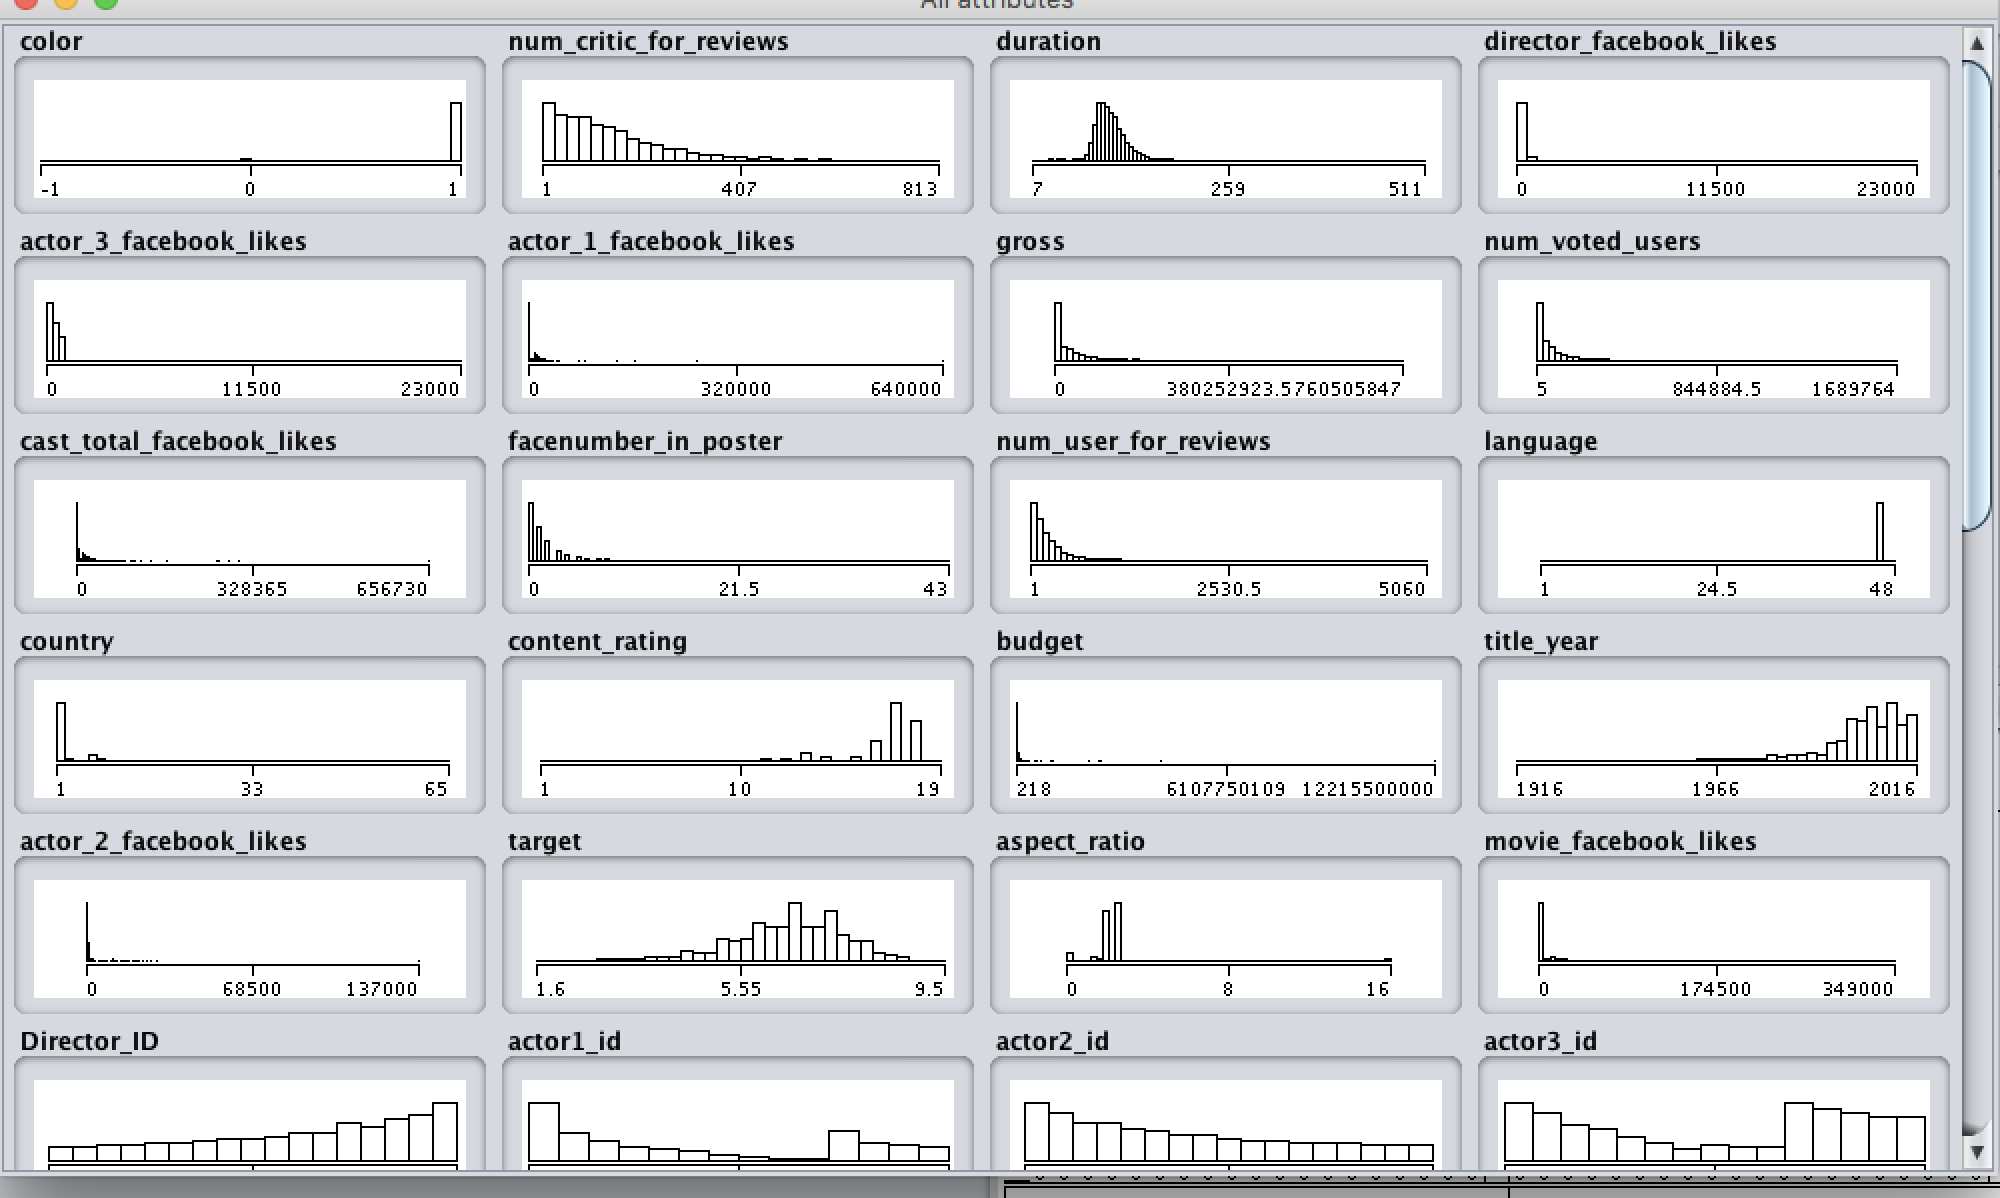
\includegraphics[height=7cm]{imagens/wekadistribuition.png}
\caption{Distribuição dos valores dos dados}
\label{distribuicao}
\end{figure}

Com o WEKA, é possível criar modelos de classificação e de clusterização, nesse caso, foi utilizado o de classificação, como mostra a figura \ref{classificationinterface}. 

\begin{figure}[H]
\centering
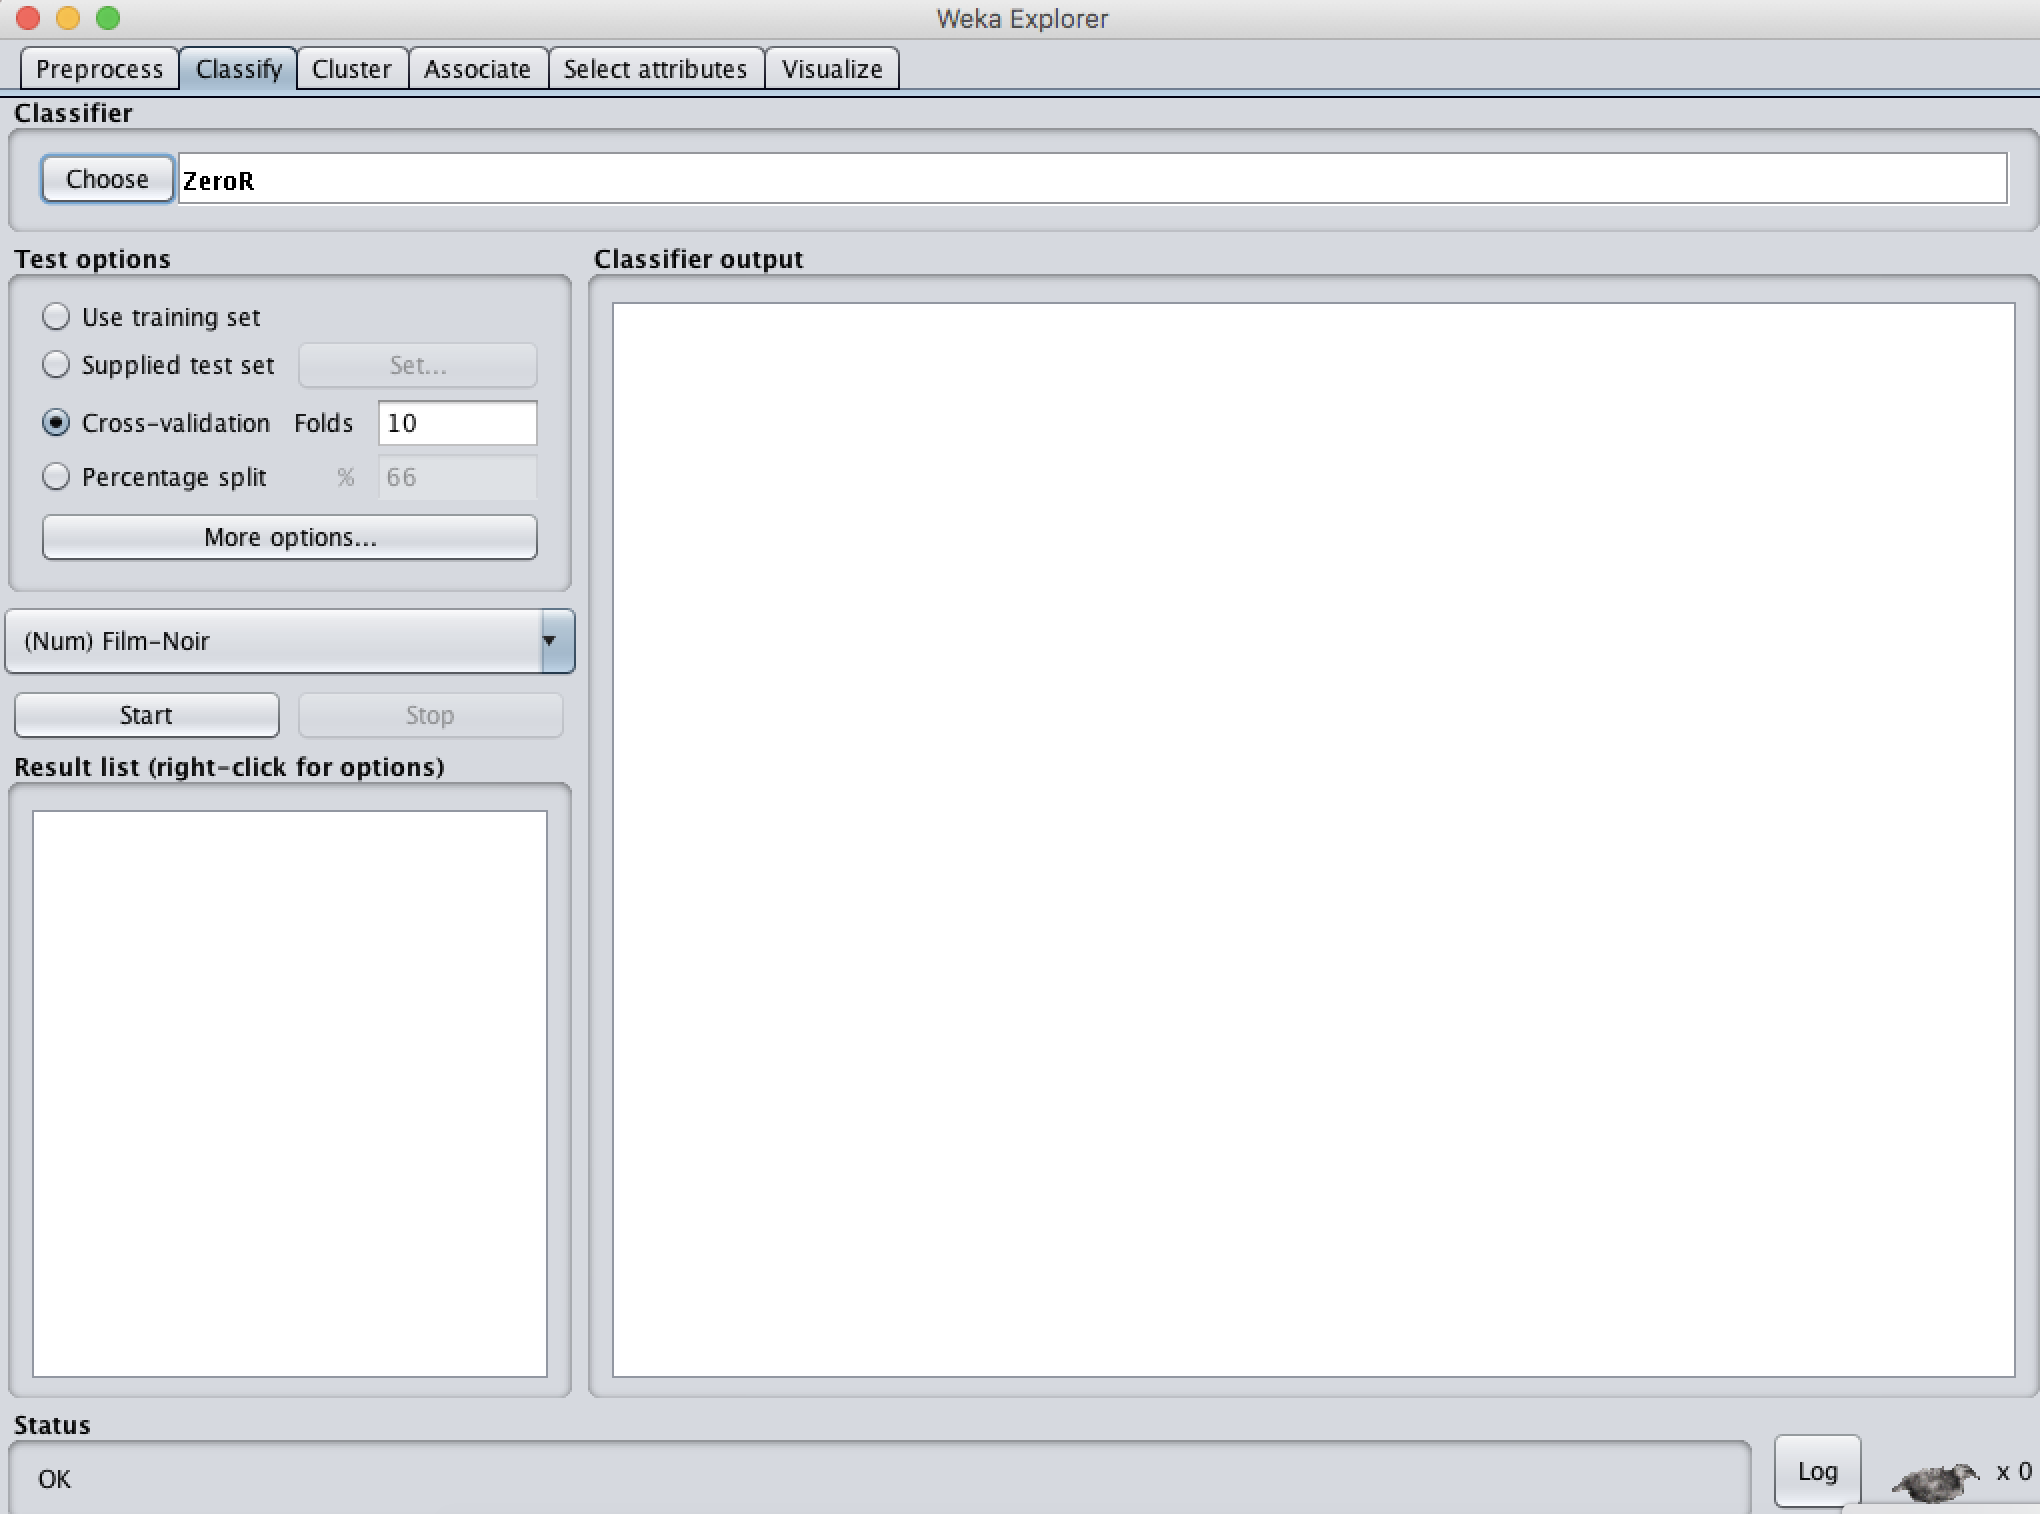
\includegraphics[height=7cm]{imagens/weka.png}
\caption{Interface de classificação}
\label{classificationinterface}
\end{figure}

Ao selecionar um algoritmo de classificação, o campo da direita irá mostrar um log do modelo, junto com o resultado encontrado.
\begin{figure}[H]
\centering
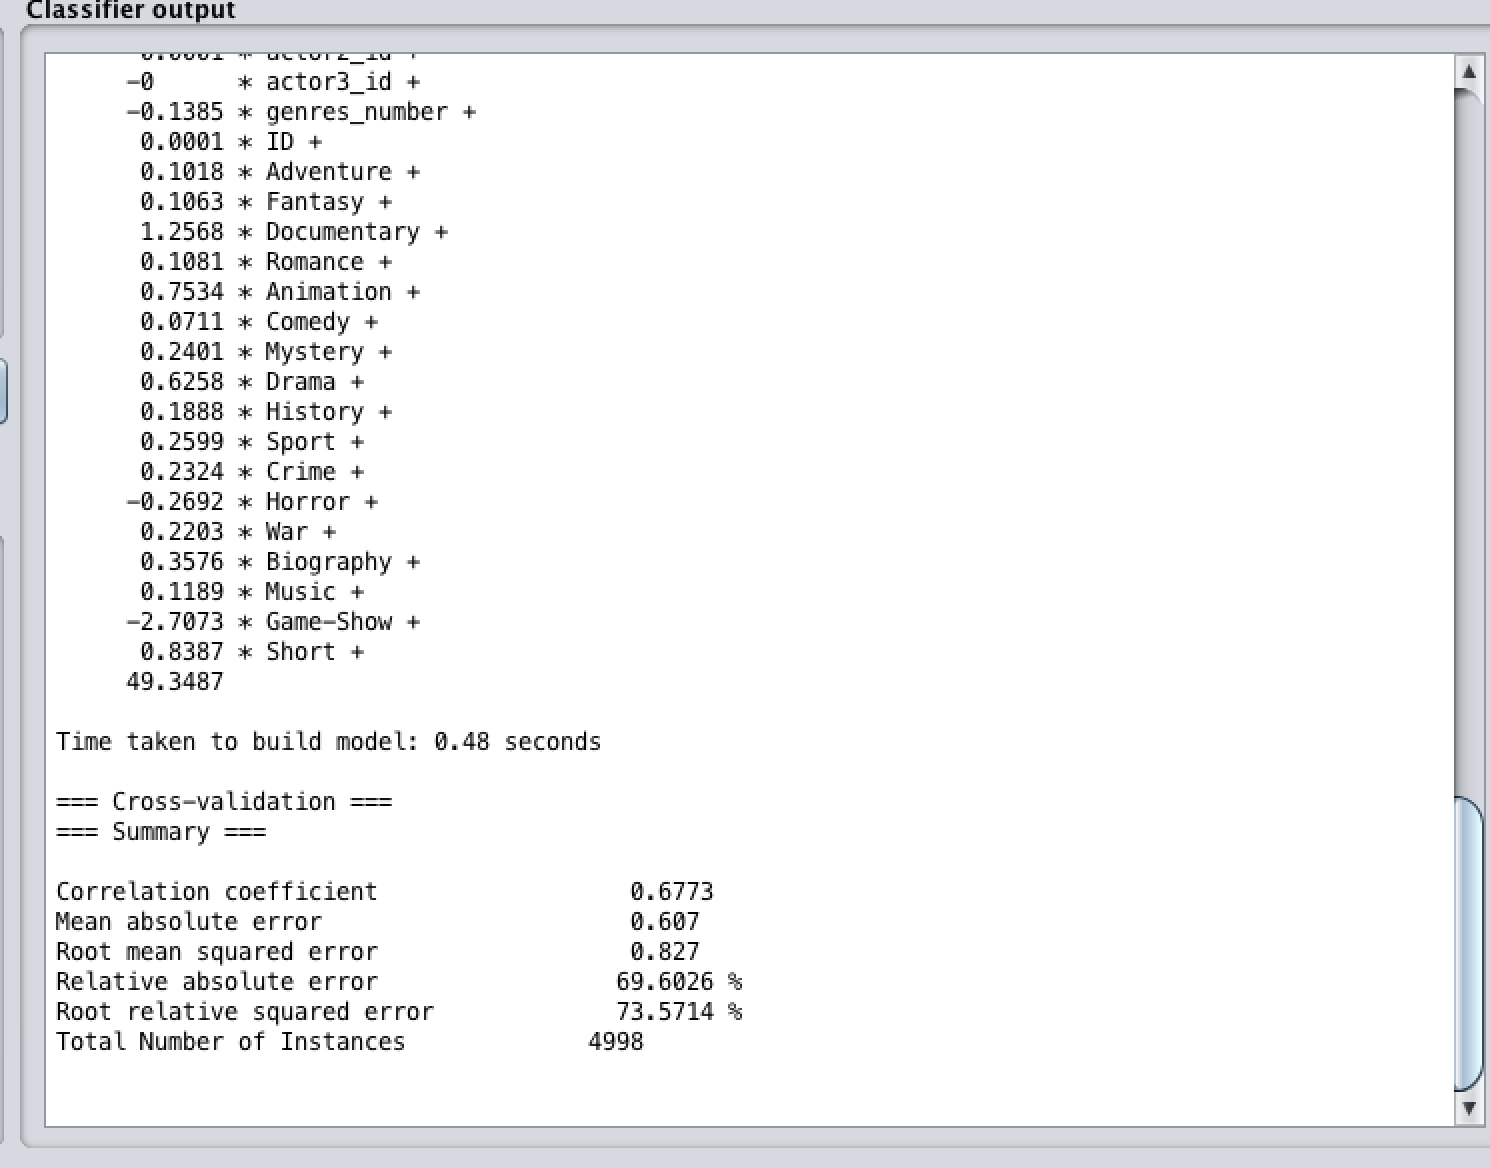
\includegraphics[height=7cm]{imagens/wekauotput.png}
\caption{Dados carregados}
\label{figura23}
\end{figure}